\documentclass[../TDE7_ocrsf.tex]{subfiles}%

\begin{document}
\section[s]"2"{Filtre de \textsc{Wien}}

\enonce{%
	\begin{minipage}{0.45\linewidth}
		On considère le circuit ci-contre avec $e(t) = E_m \cos(\wt)$. On note
		$u(t) = U_m \cos(\wt + \f)$ et on pose $H_m = U_m / E_m$ .
	\end{minipage}
	\hfill
	\begin{minipage}{0.45\linewidth}
		\begin{center}
			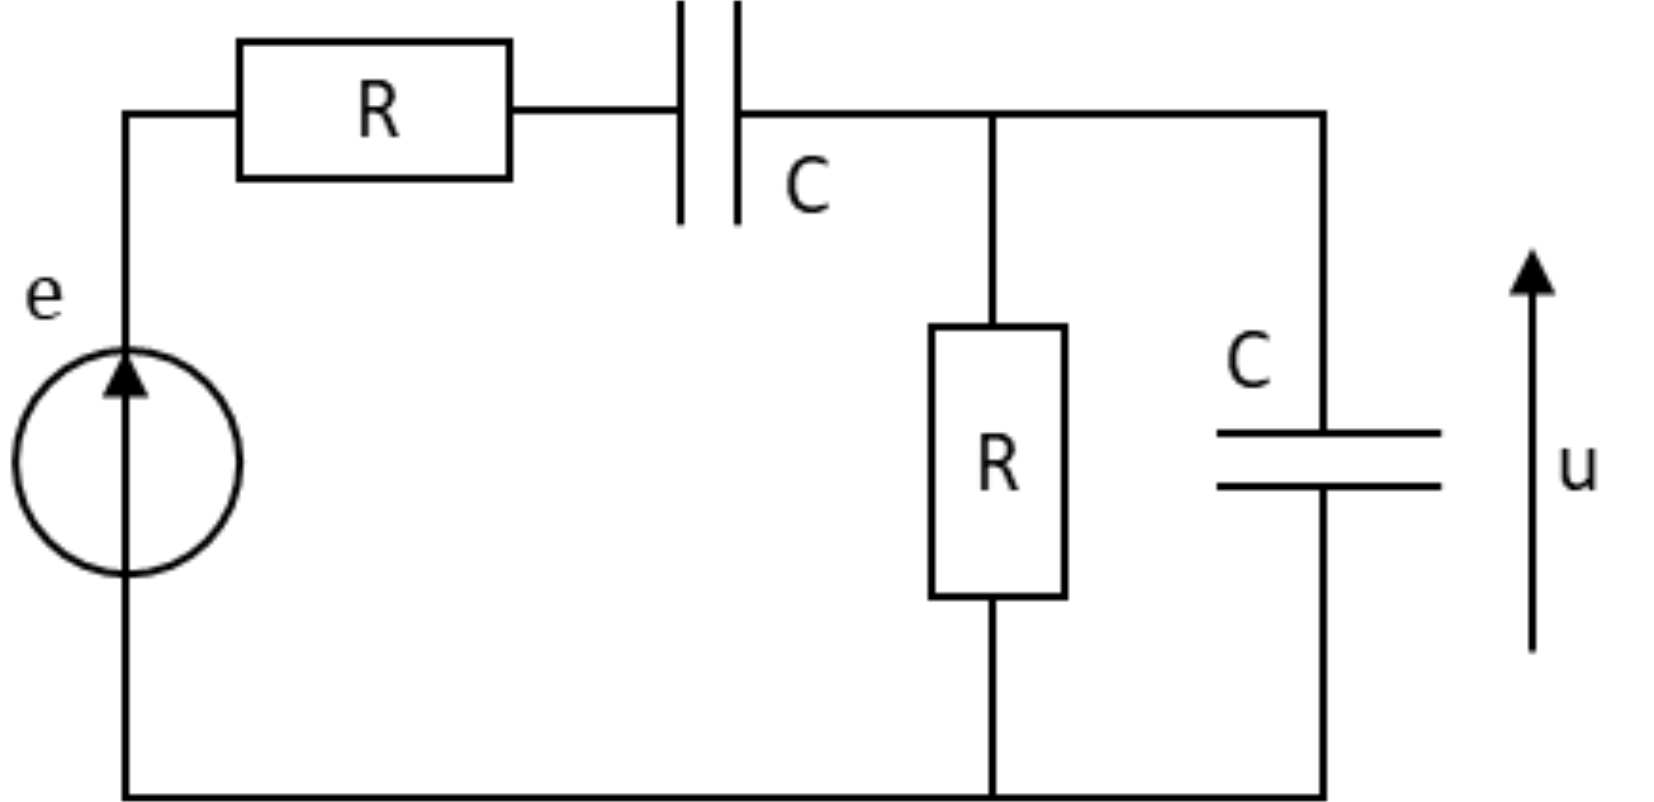
\includegraphics[width=\linewidth]{wien_1}
		\end{center}
	\end{minipage}
}
\QR{%
	Déterminer les valeurs limites de $u(t)$ à basse et haute
	fréquences.
}{%
	Dans la limite très hautes fréquences, les condensateurs sont
	équivalents à des fils, donc $\uu = 0$. Dans la limite très basses
	fréquences, les condensateurs sont cette fois équivalents à des
	interrupteurs ouverts. Aucun courant ne circule dans les résistances, et
	on a donc également $\uu = 0$. Selon toute vraisemblance, c'est donc
	un filtre \textbf{passe-bande}.
}

\enonce{%
	Les courbes représentatives de $H_m (\w)$ et $\f(\w)$ sont
	fournies par les figures ci-dessous.
	\smallbreak
	\begin{minipage}{0.45\linewidth}
		\begin{center}
			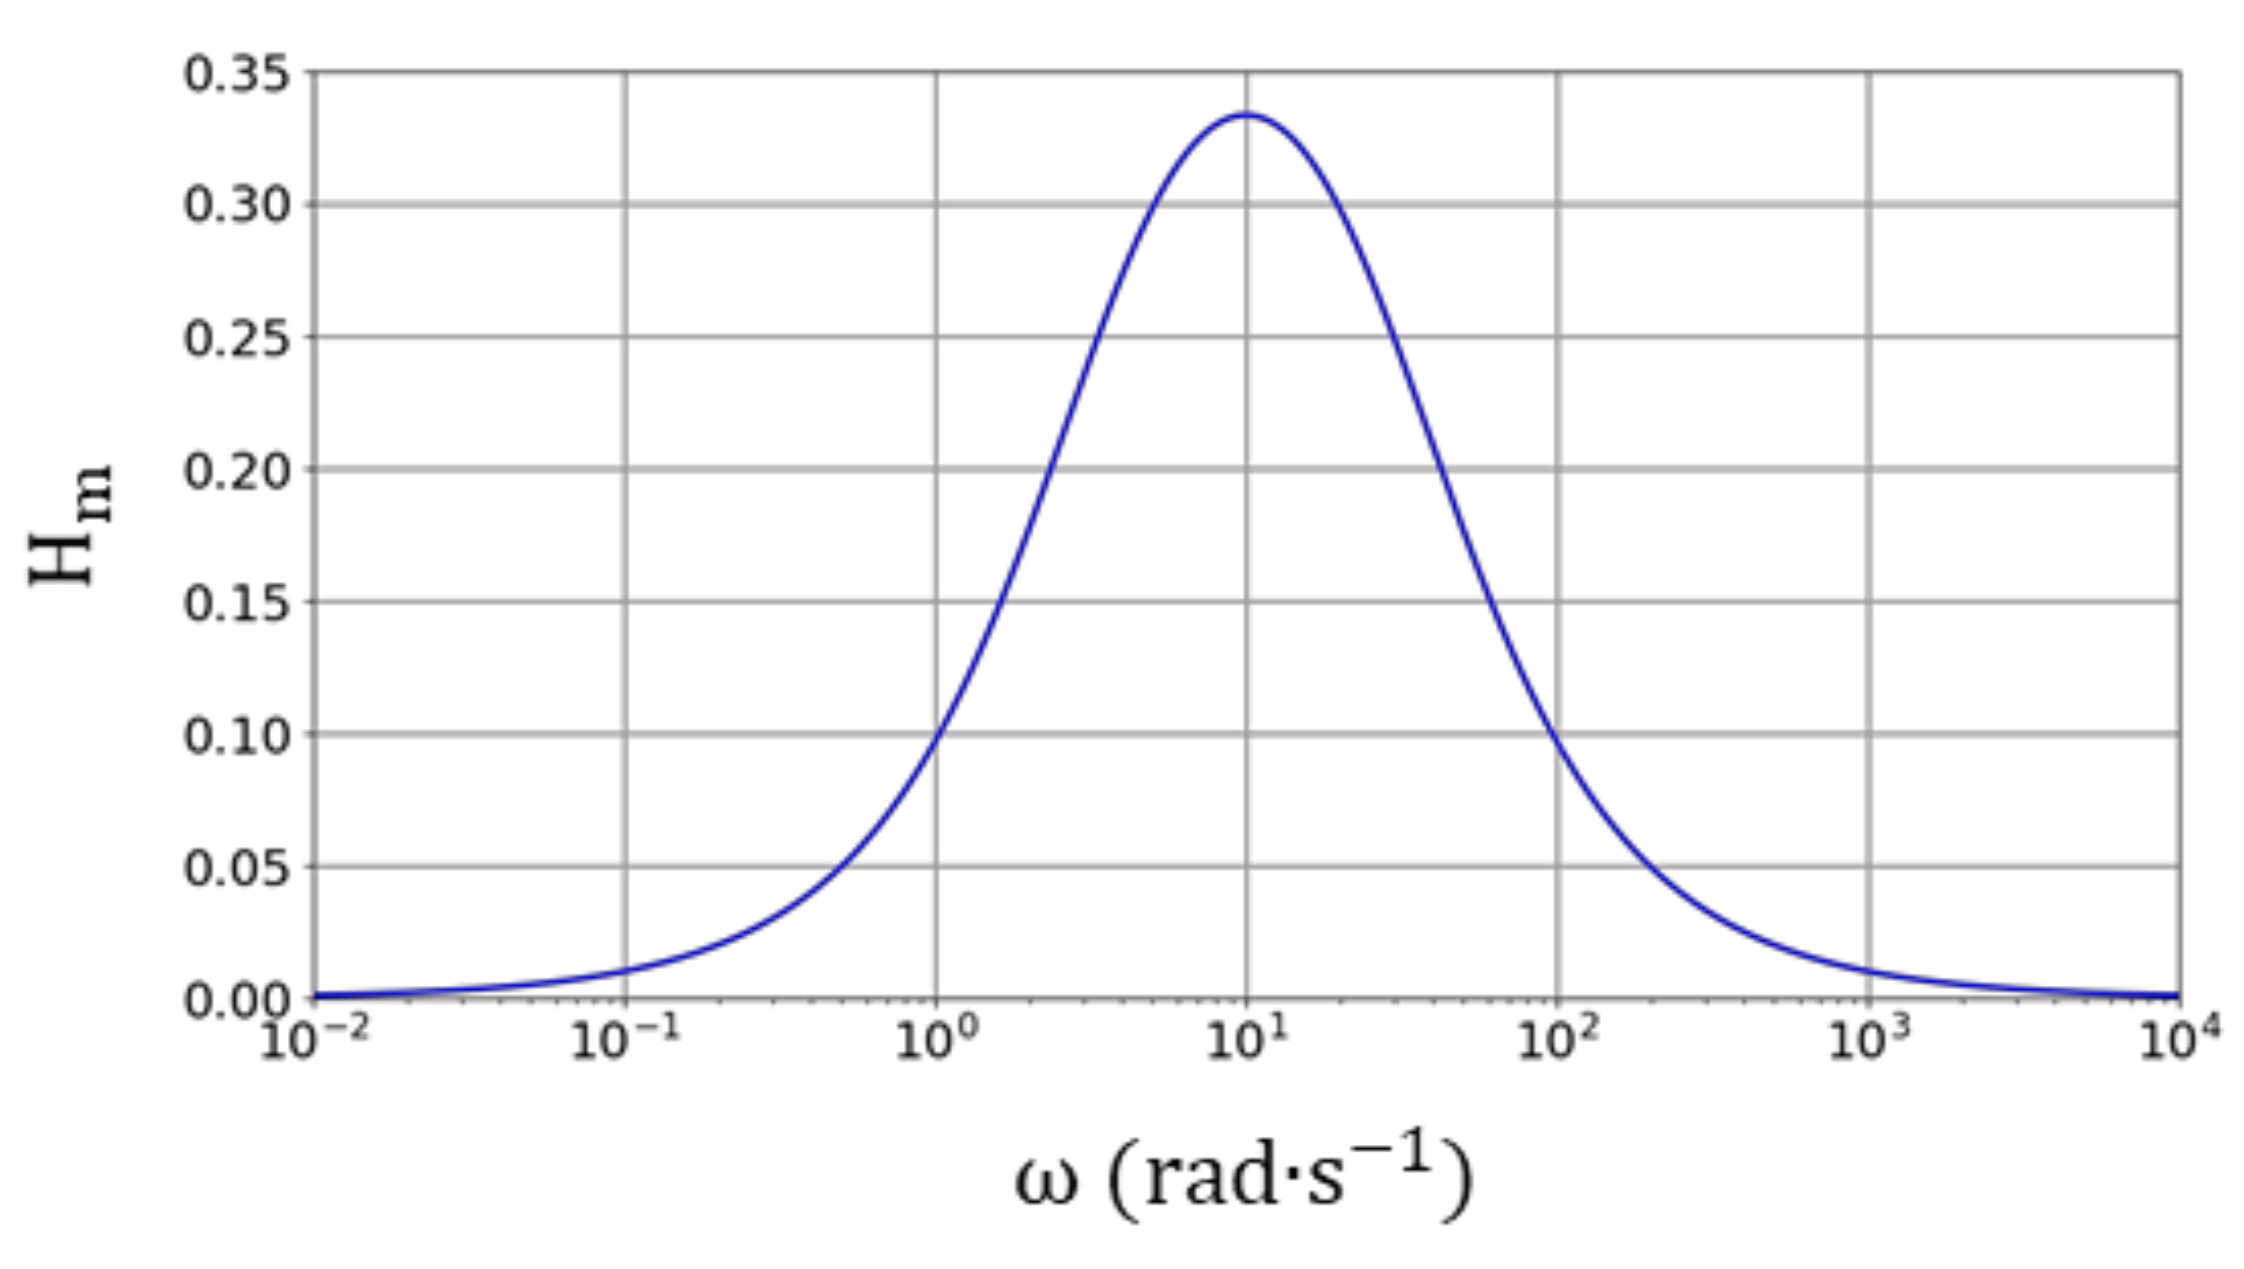
\includegraphics[width=\linewidth]{wien_3}
		\end{center}
	\end{minipage}
	\hfill
	\begin{minipage}{0.45\linewidth}
		\begin{center}
			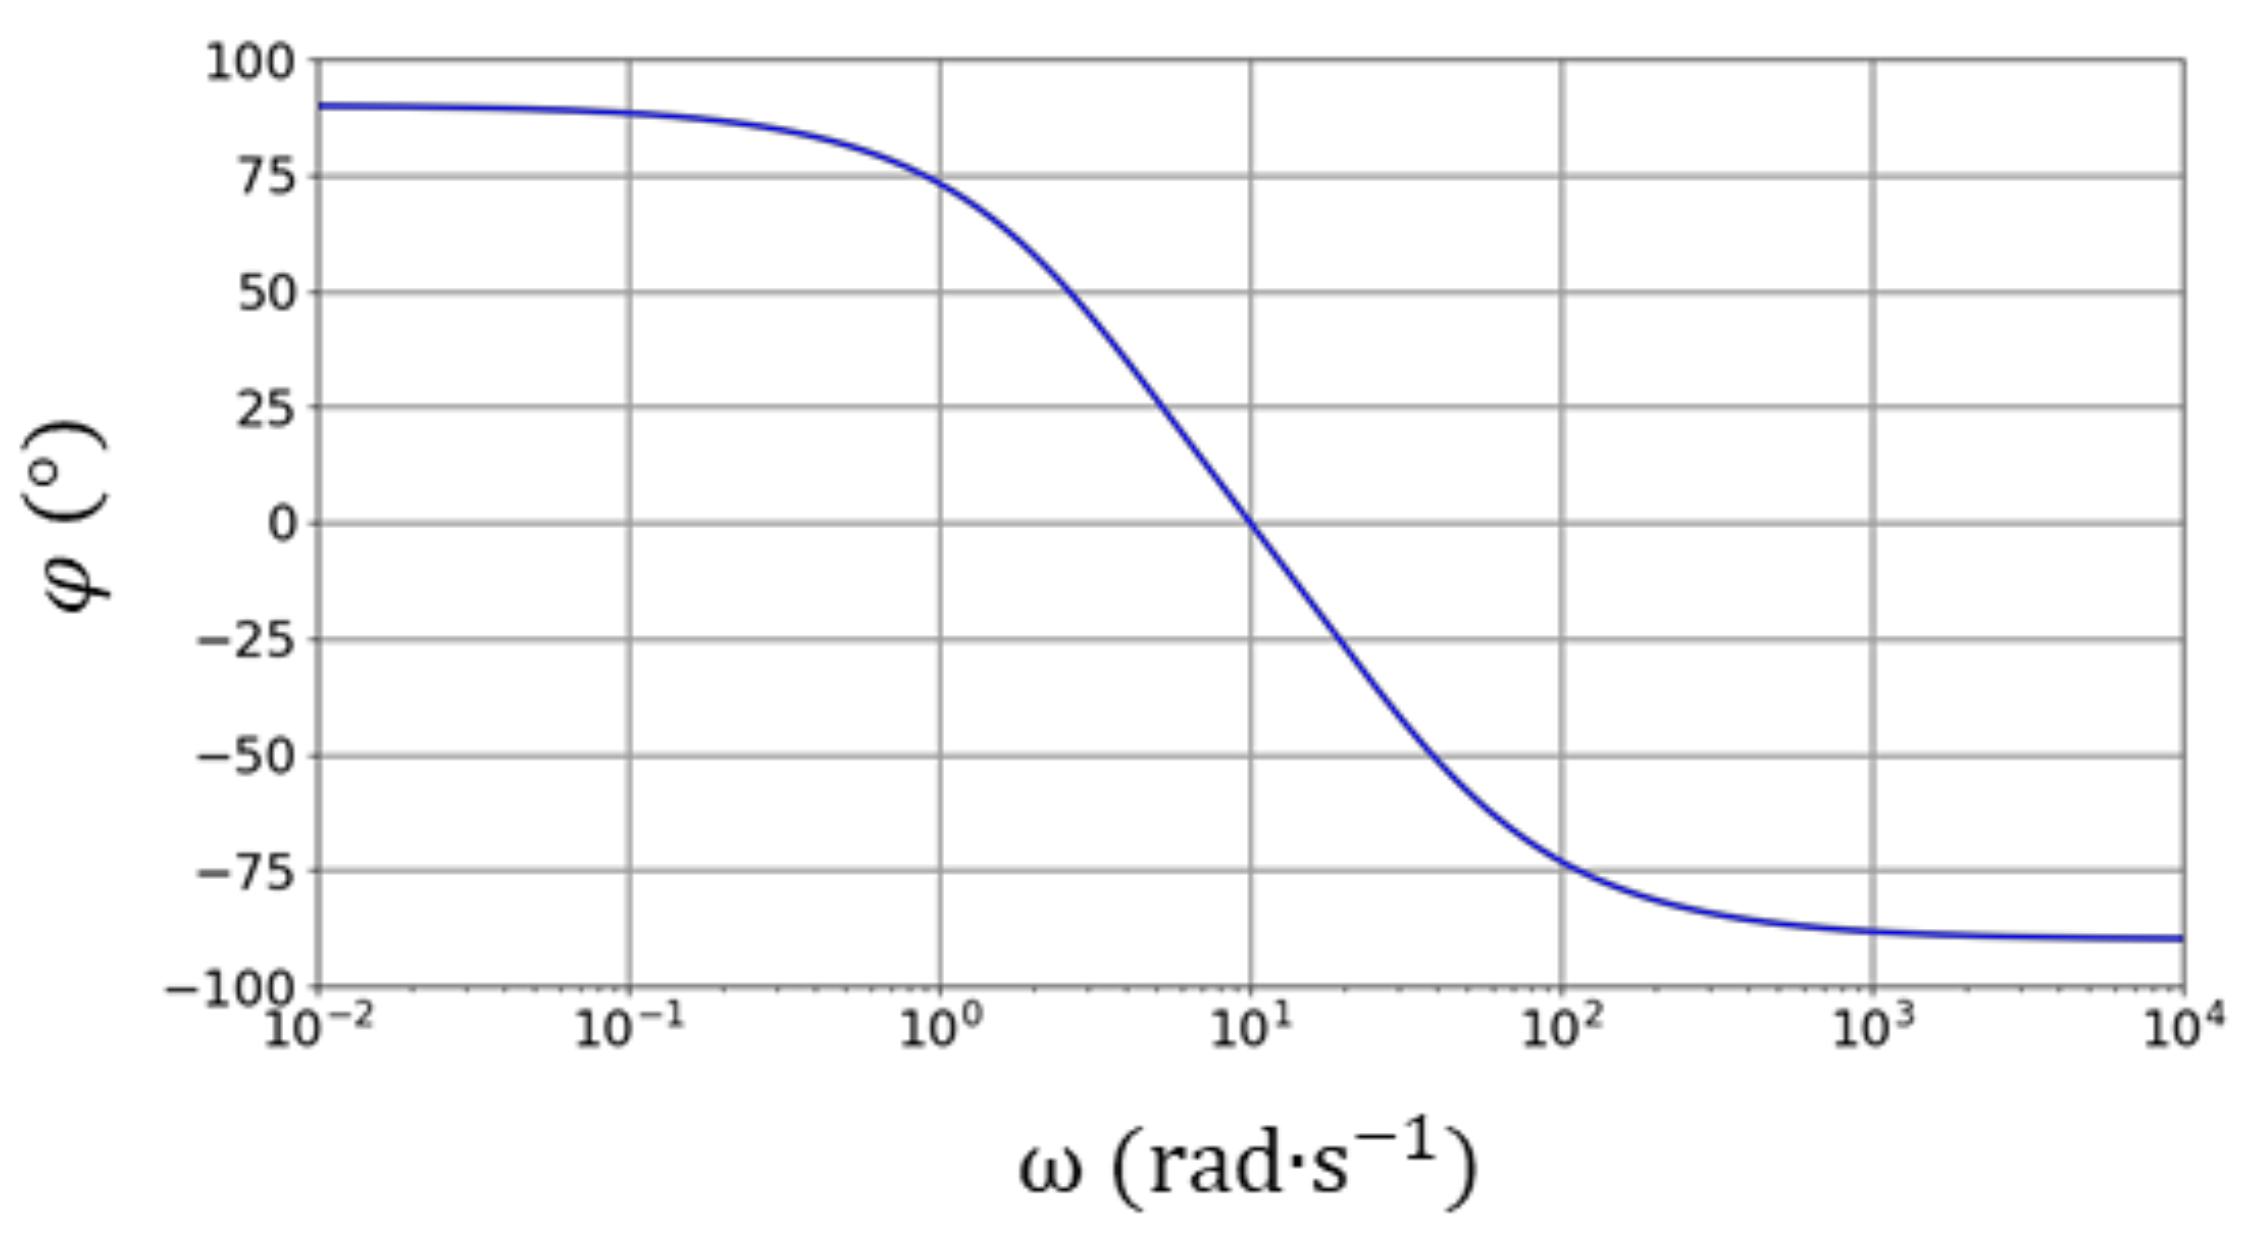
\includegraphics[width=\linewidth]{wien_2}
		\end{center}
	\end{minipage}
}

\QR{%
	Observe-t-on un phénomène de résonance en tension~? Justifier.
}{%
	On observe bien une résonance en tension, étant donné qu'on trouve un
	\textbf{maximum de l'amplitude pour $\w \neq 0$ et $\w \neq \infty$}.
}
\QR{%
	Déterminer graphiquement la pulsation de résonance, les pulsations de
	coupure et la bande passante du filtre.
}{%
	On lit \fbox{$\w_r = \SI{10}{rad.s^{-1}}$}, et on trouve les
	pulsations de coupure en traçant une droite horizontale à $H_{m,
				\max}/\sqrt{2} = \num{0.23}$ (avec $H_{m, \max} = \num{0.33}$) et en
	prenant les abscisses des intersections. On trouve alors
	\begin{gather*}
		\boxed{\w_1 = \SI{2}{rad.s^{-1}}}
		\qet
		\boxed{\w_2 = \SI{20}{rad.s^{-1}}}
		\qdonc
		\boxed{\D\w = \SI{18}{rad.s^{-1}}}
	\end{gather*}
	En effet, l'axe des abscisses est en échelle logarithmique, il faut donc
	faire attention à la lecture.
}

\QR{%
	Après avoir associé certaines impédances entre elles, établir
	l'expression de $\xul{H} = \xul{u} / \xul{e}$. La
	mettre sous la forme~:
	\[
		\xul{H}
		= \dfrac{H_0}{1 + \jj Q\left(x - \dfrac{1}{x}\right)}
		\qavec
		x = \dfrac{\w}{\w_0}
	\]
	avec $H_0$, $\w_0$ et $Q$ des constantes à exprimer en fonction
	(éventuellement) de $R$ et $C$.
}{%
	Notons $\Zu_{R\parr C}$ l'impédance et $\Yu_{R\parr C}$ l'admittance
	de l'association RC parallèle. En utilisant cette impédance, on
	reconnaît un pont diviseur de tension~:
	\begin{gather*}
		\Hu
		= \frac{\uu}{\xul{e}}
		= \frac{\Zu_{R\parr C}}{\Zu_{R\parr C} + \Zu_R + \Zu_C}
		\Leftrightarrow
		\Hu = \frac{1}{1 + \left(\Zu_R + \Zu_C\right)\Yu_{R\parr C}}\\
		\Leftrightarrow
		\xul{H}
		= \frac{1}{1 + \left(R + \dfrac{1}{\jcw}\right)\Yu_{R\parr C}}
		= \frac{1}{1 + \left(R + \dfrac{1}{\jcw}\right)\left(
			\dfrac{1}{R} + \jcw\right)}\\
		\Leftrightarrow
		\boxed{\xul{H} = \frac{1}{3+\jj\left(RC\w - \dfrac{1}{RC\w}\right)}}
	\end{gather*}
	En factorisant par 3 et en utilisant les notations introduites dans
	l'énoncé, on trouve
	\begin{gather*}
		\xul{H}
		= \frac{1/3}{1 + \dfrac{\jj}{3} \left( x - \dfrac{1}{x} \right)}
		\Leftrightarrow
		\boxed{
			\xul{H} = \frac{H_0}{1 + \jj Q \left( x - \dfrac{1}{x} \right)}}
		\qavec
		\boxed{
			\left\{
			\begin{array}{rcl}
				H_0  & = & 1/3           \\
				\w_0 & = & \dfrac{1}{RC} \\
				Q    & = & 1/3
			\end{array}
			\right.
		}
	\end{gather*}
	Ce qui est remarquable avec ce montage, c'est que \textbf{le facteur de
		qualité est de 1/3 peu importe les valeurs de $R$ et $C$}, tant que ce
	sont les mêmes $R$ et $C$ en série et en dérivation.
}

\QR{%
	Déterminer graphiquement la valeur du produit $RC$.
}{%
	Par cette étude, on trouve que $\w_r = \w_0 = \frac{1}{RC}$~; ainsi,
	on a simplement \[\boxed{RC = \SI{0.10}{Hz}}\]
}
\end{document}
